\section{第二日第三讲}

设 $F$ 是局部域 $\mathbb Q_p$、$\mathbb F_p((t))$（它们是 $2$ 维的），或者几何局部域 $\mathbb F_p((t))$（它是 $1$ 维的）。设 $O$ 是它的整数环。设 $X$ 是 $G$-簇，从而我们可以把 $X$ 看作带群 $G$ 作用的向量空间。$A_G(F)$ 是 $G(F)$-表示构成的范畴。$\Theta_X\in A_G(F)$ 是 $X(F)$ 上的函数。相对 Langlands 对应给出一个 $\check G$-簇 $\check X$ 以及 $\Theta_{\check X}\in B_{\check G}(F)$。我们想把 $\Theta_X$ 理解成一个 $G(F)$-表示，使得它在 Langlands 对应的 B 侧可以互通。

目前我们的目标是理解无分歧部分：Hecke 代数 $H:=\Hecke(G(F),G(O))$ 作用在 $X(F)$ 的 $G(O)$-不变函数上。我们想把这一作用对角化，并且要求它与来自 $X$ 的额外结构相容。先看一个模型例。

\medskip
\noindent\textbf{例 1（模型例）}\enspace
在 A 侧，我们考虑 $\mathbb Z$ 上紧支集函数构成的代数，Hecke 算子 $T$ 在它上面充当移位算子。对应的 B 侧是 Laurent 多项式环 $\mathbb C[z^{\pm1}]$。这两个代数是同构的。

在 A 侧取一个只支撑在 $0$ 上的函数，记作 $\delta_0$。对角化之后，它被送到单位元 $1\in\mathbb C[z^{\pm1}]$。A 侧 $T$ 的作用对应于 B 侧乘以 $z$。A 侧的内积 $\langle\ ,\ \rangle$ 定义为
\[
  \langle f,f\rangle=\int_{S^1}|f|^2\frac{d\theta}{2\pi},
\]
其中 $f$ 是 A 侧的函数。此外，$f$ 通过 Fourier 变换对应于 B 侧的 $\sum_n\langle f,z^n\rangle z^n\in\mathbb C[z^{\pm1}]$；反之，$g\in\mathbb C[z^{\pm1}]$ 通过逆 Fourier 变换对应于 A 侧的 $\sum_n\int_{S^1}g(z)z^n$。

取 $X=\mathbb A^1$、$G=\mathbb G_m$，则 $\mathbb A^1(F)=F$，并有赋值映射
\[
  \val:\ F/O^\times\xrightarrow{\ \sim\ }+\infty\sqcup\mathbb Z,
\]
它是同构。A 侧是 $A_G(F)=C_c(X(F))^{G(O)}$，B 侧是 $\mathbb C[\check G]=\mathbb C[\mathbb C^\times]=\mathbb C[z^{\pm1}]$。更具体地，
\begin{align*}
  C_c(X(F))^{G(O)}&=\{f:\mathbb Z\to\mathbb C:\ f(n)=\text{常数},\ n\gg0,\ f(n)=0,\ n\ll0\},\\
  H&=\mathbb C[T^{\pm1}],\quad T\ \text{是}\ \mathbb G_m(F)\ \text{中在}\ 1\ \text{处取值的元素},\\
  \delta_0&=\mathbf 1_{X(O)}=\{f=1,\ n\ge0;\ f=0,\ n<0\},\\
  \langle f,g\rangle&:=\int_F f(x)\overline{g(x)}\,dx=\sum f(n)\overline{g(n)}\,q^{-n}.
\end{align*}
% [Tutor Note: 原文说 $T$ 是 "an element of $G_m(F)$ of evaluated at 1"，语句本身残缺；按上下文应是取值（$\val$）为 1 的一致化子，译文照原文直译。]

$T$ 以下式作用在 $f$ 上：$Tf(n)=f(n+1)q^{-1/2}$。若仍用前面提到的同一个 Fourier 变换 $\langle f,z^n\rangle$，会看到 $\delta_0\in C_c(X(F))^{G(O)}$ 被送到
\[
  \frac{1}{1-q^{-1/2}z}\neq1\in\mathbb C[z^{\pm1}].
\]
为了使 $\delta_0$ 被送到 $1$，我们需要做如下重标定。构造
\[
  e_z:\ n\mapsto q^{n/2}z^n(1-q^{-1/2}z)\in C_c(X(F))^{G(O)},
\]
于是 $\delta_0\in C_c(X(F))^{G(O)}$ 被送到 $\langle\delta_0,e_z\rangle=1\in\mathbb C[z^{\pm1}]$，而 $f\in C_c(X(F))^{G(O)}$ 被送到
\[
  \langle f,e_z\rangle=\int_{S^1}|f(\theta)|^2\,d\mu
  =\int\frac{1}{(1-q^{-1/2}e^{i\theta})(1-q^{-1/2}e^{-i\theta})}\frac{d\theta}{2\pi}\in\mathbb C[z^{\pm1}].
\]

这就是模型例。接下来我们想看更一般的情形，例如球簇 $X$。

A 侧有 $\bigl(C_c(X(F))^{G(O)},\delta_0,\langle\ ,\ \rangle\bigr)$，Hecke 代数作用在 $C_c(X(F))^{G(O)}$ 上；B 侧有 $\mathbb C[Z]$，其中 $Z$ 生活在 $\check G/\mathrm{conj}$ 之上，即有映射 $Z\to\check G/\mathrm{conj}$。A 侧的 Hecke 算子可以对角化，并对应于 B 侧的乘法，这意味着每个 $z\in Z$ 给出特征 $H\to\mathbb C$。此外 $\delta_0\in C_c(X(F))^{G(O)}$ 对应于 $1\in\mathbb C[Z]$，并且 $\langle f,f\rangle=\int|f|^2\,d\mu$。

\medskip
\noindent\textbf{例 2}\enspace
考虑 $G=\mathrm{PGL}_2^l\times\mathrm{PGL}_2^r$ 作用在 $X=\mathrm{PGL}_2$ 上，其中 $l$ 表示左作用，$r$ 表示右作用。Hecke 代数是 $H=\mathbb C[T_l,T_r]$。为了理解 $X(F)/G(O)=\mathrm{PGL}_2(O)\backslash\mathrm{PGL}_2(F)/\mathrm{PGL}_2(O)$，先注意 $\mathrm{PGL}_2(F)/\mathrm{PGL}_2(O)$ 可以用 $(q+1)$-正则树的顶点来图示，如下图。
\begin{center}
  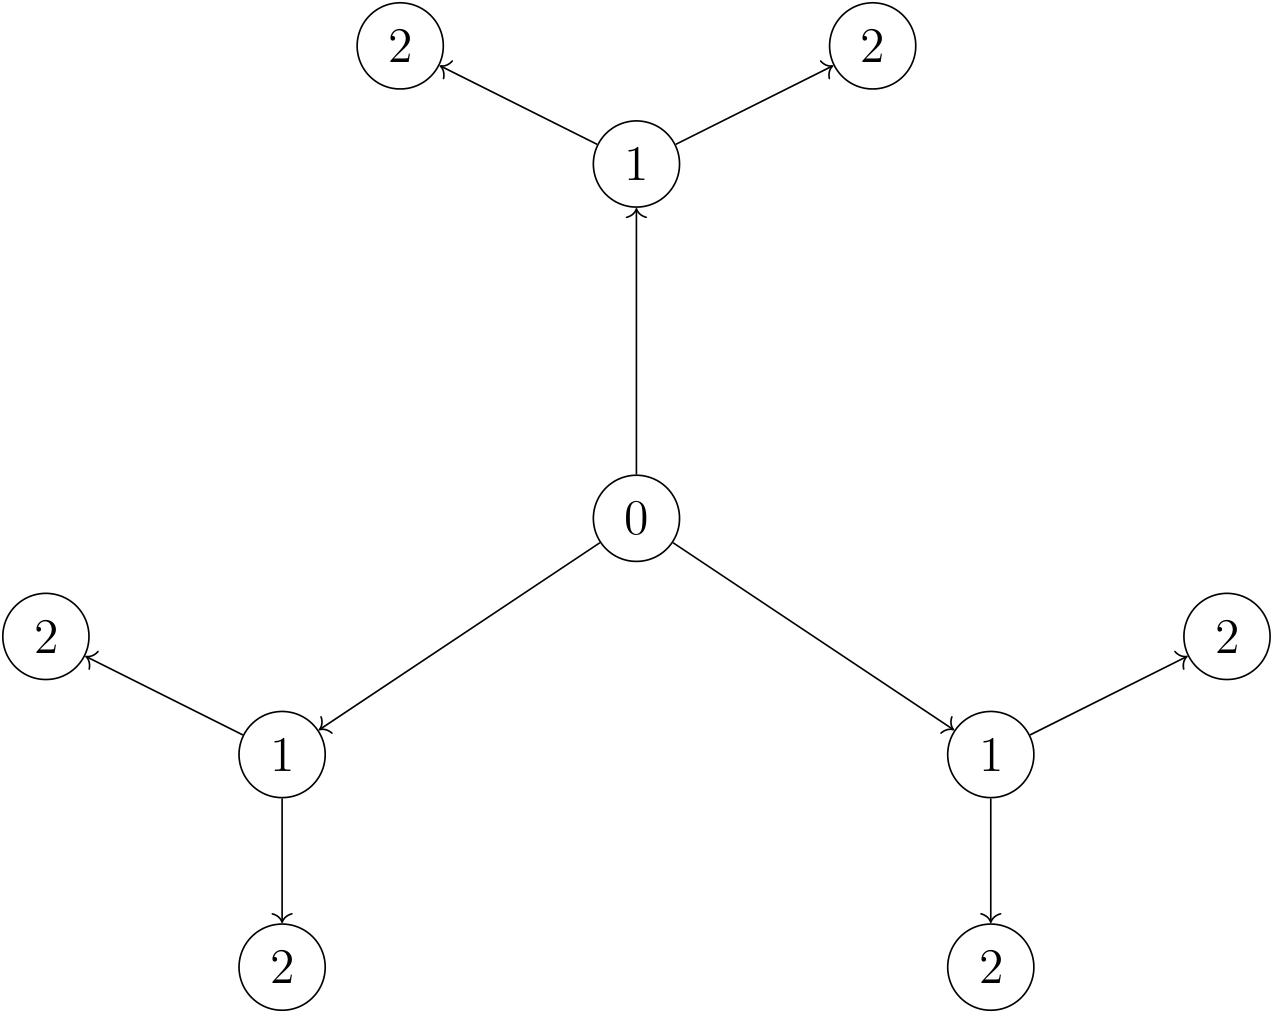
\includegraphics[width=0.36\textwidth]{figures/f61-tree.png}
\end{center}
Hecke 代数 $H(\mathrm{PGL}_2)$ 从右侧作用在它上面，Hecke 算子 $T$ 以下式作用在函数 $f$ 上：
\[
  Tf(x)=\sum_{y\sim x}f(y),
\]
其中 $x$ 是树的一个顶点，$y\sim x$ 表示与它相邻的顶点 $y$。于是对 $\mathrm{PGL}_2(O)\backslash\mathrm{PGL}_2(F)/\mathrm{PGL}_2(O)$ 有同构
\[
  X(F)/G(O)=\mathrm{PGL}_2(O)\backslash\mathrm{PGL}_2(F)/\mathrm{PGL}_2(O)\simeq\mathbb Z_{\ge0}.
\]
因此 $X(F)/G(O)$ 上的函数就是树上的径向函数。已知 $T_l=T_r$，记作 $T$。$T$ 的作用可以这样图示：固定中心顶点，让其余顶点绕中心旋转。$T$ 对函数 $f$ 的作用由下式给出
\[
  Tf(0)=(q+1)f(1),\qquad Tf(1)=f(0)+qf(2),\qquad Tf(n)=f(n-1)+qf(n+1).
\]
我们有如下对应：
\[
  C_c(X(F))^{G(O)}\longrightarrow\mathbb C[\mathrm{Sl}_2/\mathrm{conj}].
\]
左端是 A 侧，右端是 B 侧。由于 $T_l=T_r=T$（两个 Hecke 算子重合），B 侧的 $\mathrm{Sl}_2/\mathrm{conj}$ 落在 $\mathrm{Sl}_2\times\mathrm{SL}_2/\mathrm{conj}$ 的对角线上。

可以验证：A 侧的 $1$ 被送到 B 侧的 $1$；A 侧的 Hecke 算子被送到 B 侧的乘法；并且
\[
  \langle f,f\rangle=\int_{SU_2/\mathrm{conj}}f\cdot(\mathrm{SL}_2\ \text{的}\ q\text{-特征标})\cdot\text{Haar 测度},
\]
其中 $SU_2$ 是 $\mathrm{SL}_2$ 的极大紧子群。
